\chapter{Background}

Whether software engineers are aware of it or not, the programs they write are
heavily regulated by the public policy and the law. In software, the tacit
struggle between legal demands for safety and economic profitability hinders
technical progress and innovation. In isolation from one another, this chapter
explores the details of these two forces: (1) legal regulation for safety and
(2) technical innovation and profit.

\section{Legal Regulation}
\begin{quote}
``\textit{\ldots [the law], by the very necessity of its nature, is continually
transmuting those moral standards into external or objective ones\ldots}''
\flushright{\textsc{-Oliver Wendell Holmes} \cite{Holmes23}}
\end{quote}


The intent of the law is, broadly, to achieve and preserve justice 
\cite{McAdams07}. In order to assure the safety of products, the law will often
rely on common law principles \cite{Turner99}. The common law regulates based
on judgments found in previous courtroom decisions rather than on statutes
adopted by legislative bodies.

\begin{figure}[t]
\begin{center}
\includegraphics{figures/legal.eps}
\end{center}
\caption{Common Law Model}
\label{fig:commonlaw}
\end{figure}

The model in Figure \ref{fig:commonlaw} generalizes how the legal system
handles disputes (specifically disputes involving defective products) and
updates itself through an iterative feedback process. For the legal system to
be invoked, some sort of disputable accident or injury must occur. Victims who
have suffered loss will then file a lawsuit. Facts are gathered through
searching through evidence and recording testimonies. After the facts are agreed
upon, both sides will make arguments calling into question the legality of what
happened, using precedent set from previous judgments. A judge interprets what
the law states and either he or a jury decides how it will apply in each
individual case. Once a decision is rendered, a case will oftentimes go through
an appeal wherein an unsatisfied party petitions a higher court to review the
decisions of a lower court to correct errors. More arguments are made on the
legality of the previous decision, but new facts, testimony, or evidence are no
longer accepted. Once an appellate decision is made, \textit{that} holding
enters legal archives and serves as precedent for future cases.

The \textit{legal archive} consists of rulings and opinions from previous
disputes. These rulings can then be used to make decisions in the future. This
is how the common law updates itself. If an unprecedented situation comes to
suit, then the courts will have to interpret \textit{similar} situations and
apply them at the discretion of the judge.

What is noteworthy of the model in Figure \ref{fig:commonlaw} is the
retroactive application of legal decisions to each scenario. The common law is a
reactive, feedback system because only \textit{after} accident or injury occurs
will legal repercussions be dealt with in a new product's development lifecycle.
When a judgment is made, it can then be applied to future scenarios, but usually
only if a lawsuit is filed.

\subsection{Common Law Characteristics}

The common law ``\textit{is that part of the law that is within the province of
the courts themselves to establish}'' \cite{Eisenberg88}. The common law
exhibits many characteristics that make it just. Social propositions (those of
morality, policy, or experience rather than state legal rules) are enforced
impartially to any party. The courts practice a replicable system of litigation,
allowing future disputants to have recieve legal advice and planning. The common
law is also responsive to change as moral norms evolve over time 
\cite{Eisenberg88}.

Those who are affected by the common law should understand the principles of its
underpinnings. Software engineers working on safety-critical projects are
affected by the social expectations of reliable software and functional
software. But because of its unique nature, defects in software are inevitable
and typically more difficult to locate and handle than the physical flaws found
in mechanical components \cite{Parnas90}. Defects in software used in
safety-critical situations can be especially dangerous. The increasing use of
software in machines and the demand for more product functions adds complexity
and more room for error. Fortunately, the legal system can account for this
inherent complexity.

While the legal system is in place to (among other things) ensure the safety of
products, it should be noted that the law understands the costs involved in
ensuring safety measures and takes this into consideration when resolving
disputes. Scholars posit that the law balances these economic forces and ensures
safety to a reasonable cost of manufacturers \cite{Rubin77,Priest77}.

Some lawyers contend that the law evolves towards efficient decisions in 
accident disputes in courts, where ``\textit{efficient}'' in this context means
that the defendants are more likely than the victims to win the suit if an
accident occurs. This means, in terms of software engineering, that the
organization that develops a safety-critical software product will, in the long
run, tend towards winning (or possibly avoiding) dispute. This evolution towards
efficiency comes from the pressures of the litigants who have a vested interest
in the outcome of cases because they are likely to be involved in similar
disputes in the future. The party that is interested in precedent (in this
case, the defendant software development organization) will litigate until a
favorable decision is met. This means that manufacturers that are likely to be
involved in accident disputes will make preventative efforts to improve the
safety of their products so as to avoid liability in court cases \cite{Rubin77}
and more easily defend themselves in case of a dispute.

\subsection{Products Liability}

The term \textit{products liability} broadly applies to the liability of a
manufacturer or seller for injury to a buyer caused by a product that has been
sold \cite{Prosser}. A \textit{product} usually refers to physical 
merchandise that can be purchased. Officially, a product is defined as 
\begin{quote}
``\textit{\ldots tangible personal property distributed commercially for use or
consumption and other items, such as real property and electricity, when the
context of their distribution and use is sufficiently analogous to the
distribution and use of tangible personal property\ldots}(\cite{Rest3d}, 
\S19(a))''
\end{quote}

In the case of safety-critical systems, software is usually embedded in
some machine or hardware device \cite{Leveson95} that is sold as a product. When
viewed from this standpoint, software is less analogous to pure thoughts and
expressions and may be considered a product for products liability cases.

\subsection{The Court System}\label{s:courts}

The court systems in America is a highly technical and sophisticated dispute
resolution mechanism put into place to help disputants reach an agreement.
Though many disputes are settled outside of court, the court system is the
primary to set legal precedent in the common law system that pervades American
Justice. While the exact hierarchy of courts may be much more complex, the
general pattern is shown in Figure \ref{fig:courts}.

\begin{figure}[t]
\begin{center}
\includegraphics{figures/courts.eps}
\end{center}
\flushright{\footnotesize{adopted from \cite{McAdams07}}}
\caption{State and Federal Court Systems}
\label{fig:courts}
\end{figure}

The left branch of the diagram shows the state court systems. At the base are
trial courts, often referred to as district or superior courts. Most litigation
that this research is concerned with begins at the state trial courts, but
certain specialty areas (such as public utilities and workers' compensation)
have their own reserved courts \cite{McAdams07}. At this level, the trial courts
only hear a case and apply existing precedent to the case. If a disputant wishes
to appeal, he submits a request which can be heard by a higher court. Some
states provide an intermediate court of appeals between the state's highest
court and the trial courts. It as at the appeallate level that legal precedent
is set. When a judge or jury makes a decision at an appeallate court, an opinion
is written and is stored for future cases to use \cite{Eisenberg88}. If the
dispute regards a national or constitutional issue, a disputant may appeal to
the U.S. Supreme Court \cite{McAdams07}.

The middle and right branches of Figure \ref{fig:courts} provide the foundation
of the federal judicial system. A similar heirarchy exists in these branches,
but these courts hear cases involving federal law which does not include
the tortious products liability disputes that this research concerned with.

\subsection{Alternative Dispute Resolution}

The American Legal System has still yet to resolve a \textit{real} dispute
involving software. With software now being available for decades and already
causing problems worthy of litigation \cite{Therac25}, why haven't our courts
regulated for safer software?

Perhaps the reason why our courts have not addressed the issue of software
safety is because of the out-of-court measures that companies will take to
settle disputes. Often times, disputes will be settled through mediation, 
wherein a neutral third party facilitates a compromise of the situation
\cite{McAdams07}. Unfortunately, the law does not get updated through mediation
because a this kind of dispute resolution does not make a determination of right
or wrong, it merely creates a settlement and agreement not to pursue trial
litigation.

\section{Technical Evolution}

\begin{quote}
``\textit{This work must be conducted with attention to detail and the highest
standard of professional care.}''
\flushright{\textsc{-St. Jude Medical} \cite{SJMCode}}
\end{quote}

The capabilities of software have, no doubt, changed dramatically since the
introduction of computers decades ago. Society's increasing reliance on
computers and software creates pressure to adapt. Software evolves because
individuals and organizations are integrating computers into their activities
\cite{Lehman98}.

Since the audience of this research is comprised of mostly technical
intellectuals, we will only briefly discuss the cycle of innovation in software.

\begin{figure}[t]
\begin{center}
\includegraphics{figures/technical.eps}
\end{center}
\caption{Model of Technical Innovation}
\label{fig:technical}
\end{figure}

Figure \ref{fig:technical} is a broad generalization of how software evolves
over time. A client (society) demands some functionality that can best be
implemented using software. Requirements and designs are laid out, taking into
consideration the needs of the client and the current capabilities of software.
Implementors utilize the body of knowledge (software libraries) to construct the
software and contribute and new knowledge back into the library. When testing is
complete, the software is accepted and delivered.

The the evolution of software is both a proactive, feed-forward system as well
as a reactive, feedback system. Software developers use the demands of their
clients to write requirements for what they will implement. Society pushes them
to innovate and create software that will be profitable. At the same time,
testing occurs to detect errors and inadequacies and are reported back to
requirements and design planning for corrections.

\section{A Historical Analog}

The amalgamation of these two forces -- (1) the demands of our legal system to
ensure safety in products at a reasonable cost to manufacturers and (2) the
insistence of society and industry to innovate and increase profits -- is the
primary focus of this research.

History shows that the legal ramifications of products liability will limit
technical progress for for manufacturers. In the early 1990s, the small aircraft
industry observed a sharp decline in production �- from about 13,000 units at
its peak in 1977 to only 444 planes in 1994 \cite{Clancy95}. \textit{The Wall
Street Journal} argued that this decline is due, in large part, to 
products-liability laws ``\textit{eating a sick industry alive}'' 
\cite{Smith91}.

In this case, products-liability laws imposed no time limit on the support for
old products. Claims were made against companies involving planes that were
purchased decades before filing suit, causing insurance fees to climb and
scaring off investors \cite{Smith91}. When Congress responded by passing the
General Aviation Revitalization Act (GARA) in 1994, it protected companies from
serious claims involving planes older than 18 years. The risk of liability was
dramatically reduced and insurance costs were cut allowing companies like Piper
Aircraft to develop, thrive, and profit \cite{Valdmanis01}. However, reports
have shown that the alleged ``immunity'' of granted by GARA has also increased
injury related to small aircrafts \cite{Kolczynski03}.

Computer technology and software, unfortunately, has not enjoyed the same rich
history and professional research as some of the other more mature fields of
engineering. Legal disputes involving software have, thus far, not made it much
passed the trial courts and have therefore not yet been formally addressed by
the common law.
